% Options for packages loaded elsewhere
% Options for packages loaded elsewhere
\PassOptionsToPackage{unicode}{hyperref}
\PassOptionsToPackage{hyphens}{url}
\PassOptionsToPackage{dvipsnames,svgnames,x11names}{xcolor}
%
\documentclass[
]{article}
\usepackage{xcolor}
\usepackage[margin=1in]{geometry}
\usepackage{amsmath,amssymb}
\setcounter{secnumdepth}{5}
\usepackage{iftex}
\ifPDFTeX
  \usepackage[T1]{fontenc}
  \usepackage[utf8]{inputenc}
  \usepackage{textcomp} % provide euro and other symbols
\else % if luatex or xetex
  \usepackage{unicode-math} % this also loads fontspec
  \defaultfontfeatures{Scale=MatchLowercase}
  \defaultfontfeatures[\rmfamily]{Ligatures=TeX,Scale=1}
\fi
\usepackage{lmodern}
\ifPDFTeX\else
  % xetex/luatex font selection
\fi
% Use upquote if available, for straight quotes in verbatim environments
\IfFileExists{upquote.sty}{\usepackage{upquote}}{}
\IfFileExists{microtype.sty}{% use microtype if available
  \usepackage[]{microtype}
  \UseMicrotypeSet[protrusion]{basicmath} % disable protrusion for tt fonts
}{}
\makeatletter
\@ifundefined{KOMAClassName}{% if non-KOMA class
  \IfFileExists{parskip.sty}{%
    \usepackage{parskip}
  }{% else
    \setlength{\parindent}{0pt}
    \setlength{\parskip}{6pt plus 2pt minus 1pt}}
}{% if KOMA class
  \KOMAoptions{parskip=half}}
\makeatother
% Make \paragraph and \subparagraph free-standing
\makeatletter
\ifx\paragraph\undefined\else
  \let\oldparagraph\paragraph
  \renewcommand{\paragraph}{
    \@ifstar
      \xxxParagraphStar
      \xxxParagraphNoStar
  }
  \newcommand{\xxxParagraphStar}[1]{\oldparagraph*{#1}\mbox{}}
  \newcommand{\xxxParagraphNoStar}[1]{\oldparagraph{#1}\mbox{}}
\fi
\ifx\subparagraph\undefined\else
  \let\oldsubparagraph\subparagraph
  \renewcommand{\subparagraph}{
    \@ifstar
      \xxxSubParagraphStar
      \xxxSubParagraphNoStar
  }
  \newcommand{\xxxSubParagraphStar}[1]{\oldsubparagraph*{#1}\mbox{}}
  \newcommand{\xxxSubParagraphNoStar}[1]{\oldsubparagraph{#1}\mbox{}}
\fi
\makeatother


\usepackage{longtable,booktabs,array}
\usepackage{calc} % for calculating minipage widths
% Correct order of tables after \paragraph or \subparagraph
\usepackage{etoolbox}
\makeatletter
\patchcmd\longtable{\par}{\if@noskipsec\mbox{}\fi\par}{}{}
\makeatother
% Allow footnotes in longtable head/foot
\IfFileExists{footnotehyper.sty}{\usepackage{footnotehyper}}{\usepackage{footnote}}
\makesavenoteenv{longtable}
\usepackage{graphicx}
\makeatletter
\newsavebox\pandoc@box
\newcommand*\pandocbounded[1]{% scales image to fit in text height/width
  \sbox\pandoc@box{#1}%
  \Gscale@div\@tempa{\textheight}{\dimexpr\ht\pandoc@box+\dp\pandoc@box\relax}%
  \Gscale@div\@tempb{\linewidth}{\wd\pandoc@box}%
  \ifdim\@tempb\p@<\@tempa\p@\let\@tempa\@tempb\fi% select the smaller of both
  \ifdim\@tempa\p@<\p@\scalebox{\@tempa}{\usebox\pandoc@box}%
  \else\usebox{\pandoc@box}%
  \fi%
}
% Set default figure placement to htbp
\def\fps@figure{htbp}
\makeatother





\setlength{\emergencystretch}{3em} % prevent overfull lines

\providecommand{\tightlist}{%
  \setlength{\itemsep}{0pt}\setlength{\parskip}{0pt}}



 


\usepackage{float}
\usepackage{graphicx}
\usepackage{fancyhdr}
\AtBeginDocument{\pagenumbering{gobble}}
\makeatletter
\@ifpackageloaded{caption}{}{\usepackage{caption}}
\AtBeginDocument{%
\ifdefined\contentsname
  \renewcommand*\contentsname{Table of contents}
\else
  \newcommand\contentsname{Table of contents}
\fi
\ifdefined\listfigurename
  \renewcommand*\listfigurename{List of Figures}
\else
  \newcommand\listfigurename{List of Figures}
\fi
\ifdefined\listtablename
  \renewcommand*\listtablename{List of Tables}
\else
  \newcommand\listtablename{List of Tables}
\fi
\ifdefined\figurename
  \renewcommand*\figurename{Figure}
\else
  \newcommand\figurename{Figure}
\fi
\ifdefined\tablename
  \renewcommand*\tablename{Table}
\else
  \newcommand\tablename{Table}
\fi
}
\@ifpackageloaded{float}{}{\usepackage{float}}
\floatstyle{ruled}
\@ifundefined{c@chapter}{\newfloat{codelisting}{h}{lop}}{\newfloat{codelisting}{h}{lop}[chapter]}
\floatname{codelisting}{Listing}
\newcommand*\listoflistings{\listof{codelisting}{List of Listings}}
\makeatother
\makeatletter
\makeatother
\makeatletter
\@ifpackageloaded{caption}{}{\usepackage{caption}}
\@ifpackageloaded{subcaption}{}{\usepackage{subcaption}}
\makeatother
\usepackage{bookmark}
\IfFileExists{xurl.sty}{\usepackage{xurl}}{} % add URL line breaks if available
\urlstyle{same}
\hypersetup{
  colorlinks=true,
  linkcolor={blue},
  filecolor={Maroon},
  citecolor={Blue},
  urlcolor={Blue},
  pdfcreator={LaTeX via pandoc}}


\author{}
\date{}
\begin{document}

\begin{titlepage}
\centering
\vspace*{2cm}
{\Huge\bfseries Epidemiological Modeling: Spatial SIR (PDE) Model\par}
\vspace{1cm}
{\Large Project Report Mathematical Modelling; ACLS AS25\par}
\vspace{2cm}
{\large Noirin Graham, Kai Aebli\par}
\vspace{0.5cm}
{\large 2026-01-19\par}
\vfill
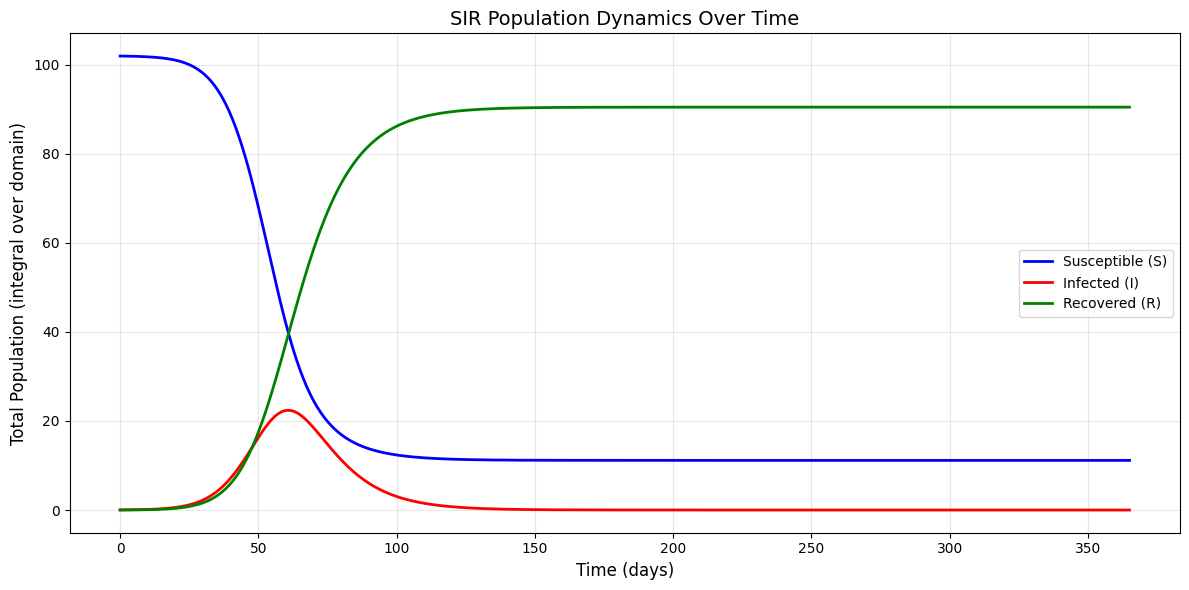
\includegraphics[width=0.9\textwidth]{images/Model_over_time.png}
\vspace{1cm}
{\large SIR-Model: S, I, R over time\par}
\vfill
\end{titlepage}
\newpage
\tableofcontents
\newpage
\pagenumbering{arabic}


\section{Introduction}\label{introduction}

In this project we consider a spatial version of the
Susceptible-Infectious-Recovered (SIR) model. \ldots{} Maybe not needed
?

\section{Model Formulation}\label{model-formulation}

We consider a spatially distributed population in two dimensions over
time and model the spread of an infectious disease. The population
density \(N(x,y,t)\) is conserved and composed of three compartments:
Susceptible \((S)\), Infectious \((I)\), and Recovered \((R)\). The PDE
system is given by:

\begin{align}
\frac{\partial S}{\partial t} &= D_s \nabla^2 S -\beta \frac{S I}{N}, \tag{1}\\
\frac{\partial I}{\partial t} &= D_i \nabla^2 I + \beta \frac{S I}{N} - \gamma I, \tag{2}\\
\frac{\partial R}{\partial t} &= \gamma I. \tag{3}
\end{align}

With the following parameters:

\begin{itemize}
\tightlist
\item
  \(\beta > 0\): transmission rate (time\(^{-1}\))\\
\item
  \(\gamma > 0\): recovery rate (time\(^{-1}\))\\
\item
  \(D_s \ge 0\): diffusion coefficient of susceptible individuals
  (space\(^2\)/time)
\item
  \(D_i \ge 0\): diffusion coefficient of infected individuals
  (space\(^2\)/time)
\end{itemize}

The infection term \(\beta \frac{SI}{N}\) transfers individuals from
\(S\) to \(I\), and the recovery term \(\gamma I\) transfers individuals
from \(I\) to \(R\). The diffusion terms in \(S\) and \(I\) model random
movement of individuals, leading to the spatial spread of the disease.

The spatial SIR model defined by equations 1 to 3 is a time-dependent,
non-linear reaction-diffusion system. The laplacian operator
\(\nabla^2\) in the diffusion terms make the system second-order and the
coupling term \(\beta \frac{SI}{N}\) makes it non-linear, as the
dependent variables \(S\) and \(I\) are mutliplied.

\section{Model Assumptions and
Choices}\label{model-assumptions-and-choices}

To simulate the system, we make the following assumptions and choices:

\begin{itemize}
\tightlist
\item
  Finite Difference Scheme: We employ the Forward-Time Central-Space
  (FTCS) scheme. This explicit method simulates the state at \(t_i\)
  directly from the known values at \(t_{i-1}\), while spatial
  derivatives (\(\nabla^2\)) are approximated using the central finite
  difference method.
\item
  Boundary Conditions: We assume an isolated population with no movement
  in or out of the defined space. This is enforced with Neumann boundary
  conditions (no-flux is implemented by equating boundary values to
  their neighbouring interior values) to the compartments \(S\) and
  \(I\) - \(R\) does not diffuse.
\item
  Initial Conditions: The model is initialized with a uniformly
  distributed susceptible population and a small localized concentration
  of infected individuals \((I)\) is planted in the center of the grid
  to simulate the outbreak.
\item
  Parameter Choices: Model parameters are assumed to be constant.
  Separate diffusion coefficients allow to model different behaviours of
  Susceptible \((S)\) and Infected \((I)\) individuals. Parameter values
  are chosen based on the given typical values in the project
  description and varied to explore their influence on the model.
\end{itemize}

CITATION LEVEQUE AND
https://www.medrxiv.org/content/10.1101/2020.06.24.20139071v2.full

\section{Discretisation}\label{discretisation}

Space is discretised on a uniform grid with spacings
\(h = \Delta x = \Delta y\) and time with step size \(\Delta t\). The
differential operators are approximated as follows:

\begin{itemize}
\tightlist
\item
  Spatial Discretisaton: The Laplacian operator \(\nabla^2 u\) in the
  diffusion term is approximated using a five-point stencil, which is
  second-order accurate. For any grid point (i,j):
\end{itemize}

\[
\Delta^2u_{i,j} \approx \frac{u_{i+1,j}+u_{i-1,j}+ u_{i,j+1}+u_{i,j-1}-4u_{i,j}}{h^2}
\]

\begin{itemize}
\tightlist
\item
  Time Stepping: We use the explicit Forward Euler method to advance the
  solution in time. Following the general discrete-time formulation
  \(x_{n+1}=f(x_n)\) the state at the next time step is computed
  directly from the current values: \[
  u^{n+1} = u^n + \Delta t \cdot \frac{\partial u^n}{\partial t}
  \]
\end{itemize}

Numerical boundary conditions are enforced by the previosuly mentioned
Neumann boundary conditions.

\section{Stability and Error
Analysis}\label{stability-and-error-analysis}

\begin{itemize}
\item
  Step-wise Order of Error: The FTCS scheme combines a forward
  difference in time (\(\mathcal{O}(\Delta t)\)) and a central
  difference in space (\(\mathcal{O}(h^2)\)). Hence, the local
  truncation error of the approximation scales like
  \(\mathcal{O}(\Delta t,h^2)\).
\item
  Stability Condition: As an explicit method, the FTCS scheme is only
  conditionally stable. To ensure numerical stability, the time step
  \(\Delta t\) is constrained by the diffusion limit (the time step must
  be sufficiently small relative to the spatial grid size):
  \(\Delta t \le \frac{1}{2D\left(\frac{1}{\Delta x^2} + \frac{1}{\Delta y^2}\right)}\)

  This restriction follows from a method of lines stability analysis.
  Spatial discretisation of the diffusion term leads to a linear ODE
  system \(\dot{\mathbf{u}} = D\,L\,\mathbf{u}\), where \(L\) is the
  discrete Laplacian matrix. For Forward Eulor time integration is
  stable only if the condition \(1 + \Delta t\,D\,\lambda \in [-1,1]\)
  is satisfied for all eigenvalues \(\lambda\) of \(L\), whose largest
  magnited scales as \(4(\Delta x^{-2} + \Delta y^{-2})\), yielding the
  stated restriction on \(\Delta t\). In our implementation an
  additional safety factor of \(0.5\) to this limit.
\end{itemize}

\section{Implementation}\label{implementation}

The model simulates disease spread across a 100×100 grid using the
finite difference method. Rather than treating the population as one
large group, it tracks how the disease spreads spatially, as if
observing it move across a map. Each cell tracks susceptible (S),
infected (I), and recovered (R) populations. Diffusion between
neighbouring cells is controlled by coefficients \(D_s\) and \(D_i\),
with zero-flux Neumann boundaries.

\subsection{Initial Conditions Setup}\label{initial-conditions-setup}

Separate grids were created for each state (S, I and R). The infected
population (1\% of total) was initialized at the grid center using a
Gaussian distribution, with susceptible individuals (99\%) uniformly
distributed and recovered population initially zero.

\subsection{Time stepping routine}\label{time-stepping-routine}

The model uses the Euler method, following a step-wise approach. The
time step was chosen to ensure numerical stability. The maximum stable
time step was calculated as
\(dt_{\text{max}} = \frac{1}{2 \cdot D_{\text{max}} \cdot (\frac{1}{dx^2} + \frac{1}{dy^2})}\).
The actual time step used was \(dt = 0.5 \times dt_{\text{max}}\),
incorporating a safety factor of 0.5 to prevent the solution from
becoming unstable during the simulation.

At each time step implemented in the sir\_step function, Neumann
boundary conditions were applied to the susceptible and infected
populations. The total population was calculated as \(N = S + I + R\),
and the reaction terms for infection (\(\beta \frac{SI}{N}\)) and
recovery (\(\gamma I\)), as well as the diffusion terms (\(\nabla^2 S\)
and \$\textbackslash nabla\^{}2 I\$), were computed using finite
differences.

All populations were then updated according to
\(S^{n+1} = S^n + dt \cdot (D_s \nabla^2 S - \text{infection})\),
\(I^{n+1} = I^n + dt \cdot (D_i \nabla^2 I + \text{infection} - \text{recovery})\),
and \(R^{n+1} = R^n + dt \cdot \text{recovery}\). Any negative values
were set to zero to ensure physical validity.

\subsection{Simulation of the PDE}\label{simulation-of-the-pde}

The simulation was initiated by the \texttt{run\_simulation} function,
which combined all the model's components. This function initialised the
spatial grids with the defined initial conditions and set the
epidemiological parameters (\(\beta\) and \(\gamma\)) and the diffusion
coefficients (\(D_s\) and \(D_i\)). Four scenarios were simulated over
365 days (\textasciitilde73,000 steps). Snapshots were saved every 50
steps for analysis.

\begin{longtable}[]{@{}
  >{\raggedright\arraybackslash}p{(\linewidth - 6\tabcolsep) * \real{0.2500}}
  >{\raggedright\arraybackslash}p{(\linewidth - 6\tabcolsep) * \real{0.2500}}
  >{\raggedright\arraybackslash}p{(\linewidth - 6\tabcolsep) * \real{0.2500}}
  >{\raggedright\arraybackslash}p{(\linewidth - 6\tabcolsep) * \real{0.2500}}@{}}
\toprule\noalign{}
\begin{minipage}[b]{\linewidth}\raggedright
Scenario 1
\end{minipage} & \begin{minipage}[b]{\linewidth}\raggedright
Scenario 2
\end{minipage} & \begin{minipage}[b]{\linewidth}\raggedright
Scenario 3
\end{minipage} & \begin{minipage}[b]{\linewidth}\raggedright
Scenario 4
\end{minipage} \\
\midrule\noalign{}
\endhead
\bottomrule\noalign{}
\endlastfoot
low \(\beta\) low \(\gamma\) & high \(\beta\) low \(\gamma\) & low
\(\beta\) high \(\gamma\) & high \(\beta\) high \(\gamma\) \\
\end{longtable}

\section{Stability Investigation}\label{stability-investigation}

\begin{figure}[H]

{\centering \pandocbounded{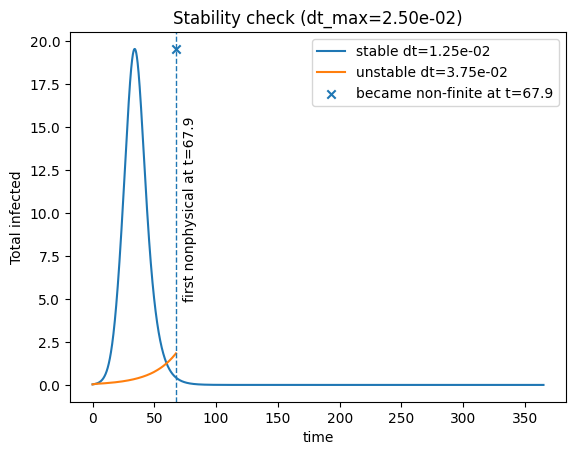
\includegraphics[keepaspectratio]{images/stability_check.png.png}}

}

\caption{Stability investigation by increasing the time step}

\end{figure}%

dt\_max detlat

Grid x 0.15 (lösung nicht mehr stimmen)

\section{Parameter Studies}\label{parameter-studies}

The following plot shows the impact of different transmission
(\(\beta\)) and recovery (\(\gamma\)) rates on the spatial dynamics.
Each row shows a different scenario. These scenarios are described in
the section ``Simulation of the PDE''. Each column shows a different
day. The countdown begins at day 0 and ends at day 365. Each scenario
begins with a small number of infected individuals in the middle.

The plot clearly shows that when transmission is low and the recovery
rate is high, the number of infected people on the last day was the
highest. It can be observed that a high transmission causes the disease
to spread faster towards the edges, while a low transmission keeps the
infected population for a longer time concentrated in the middle.

\begin{figure}[H]

{\centering \pandocbounded{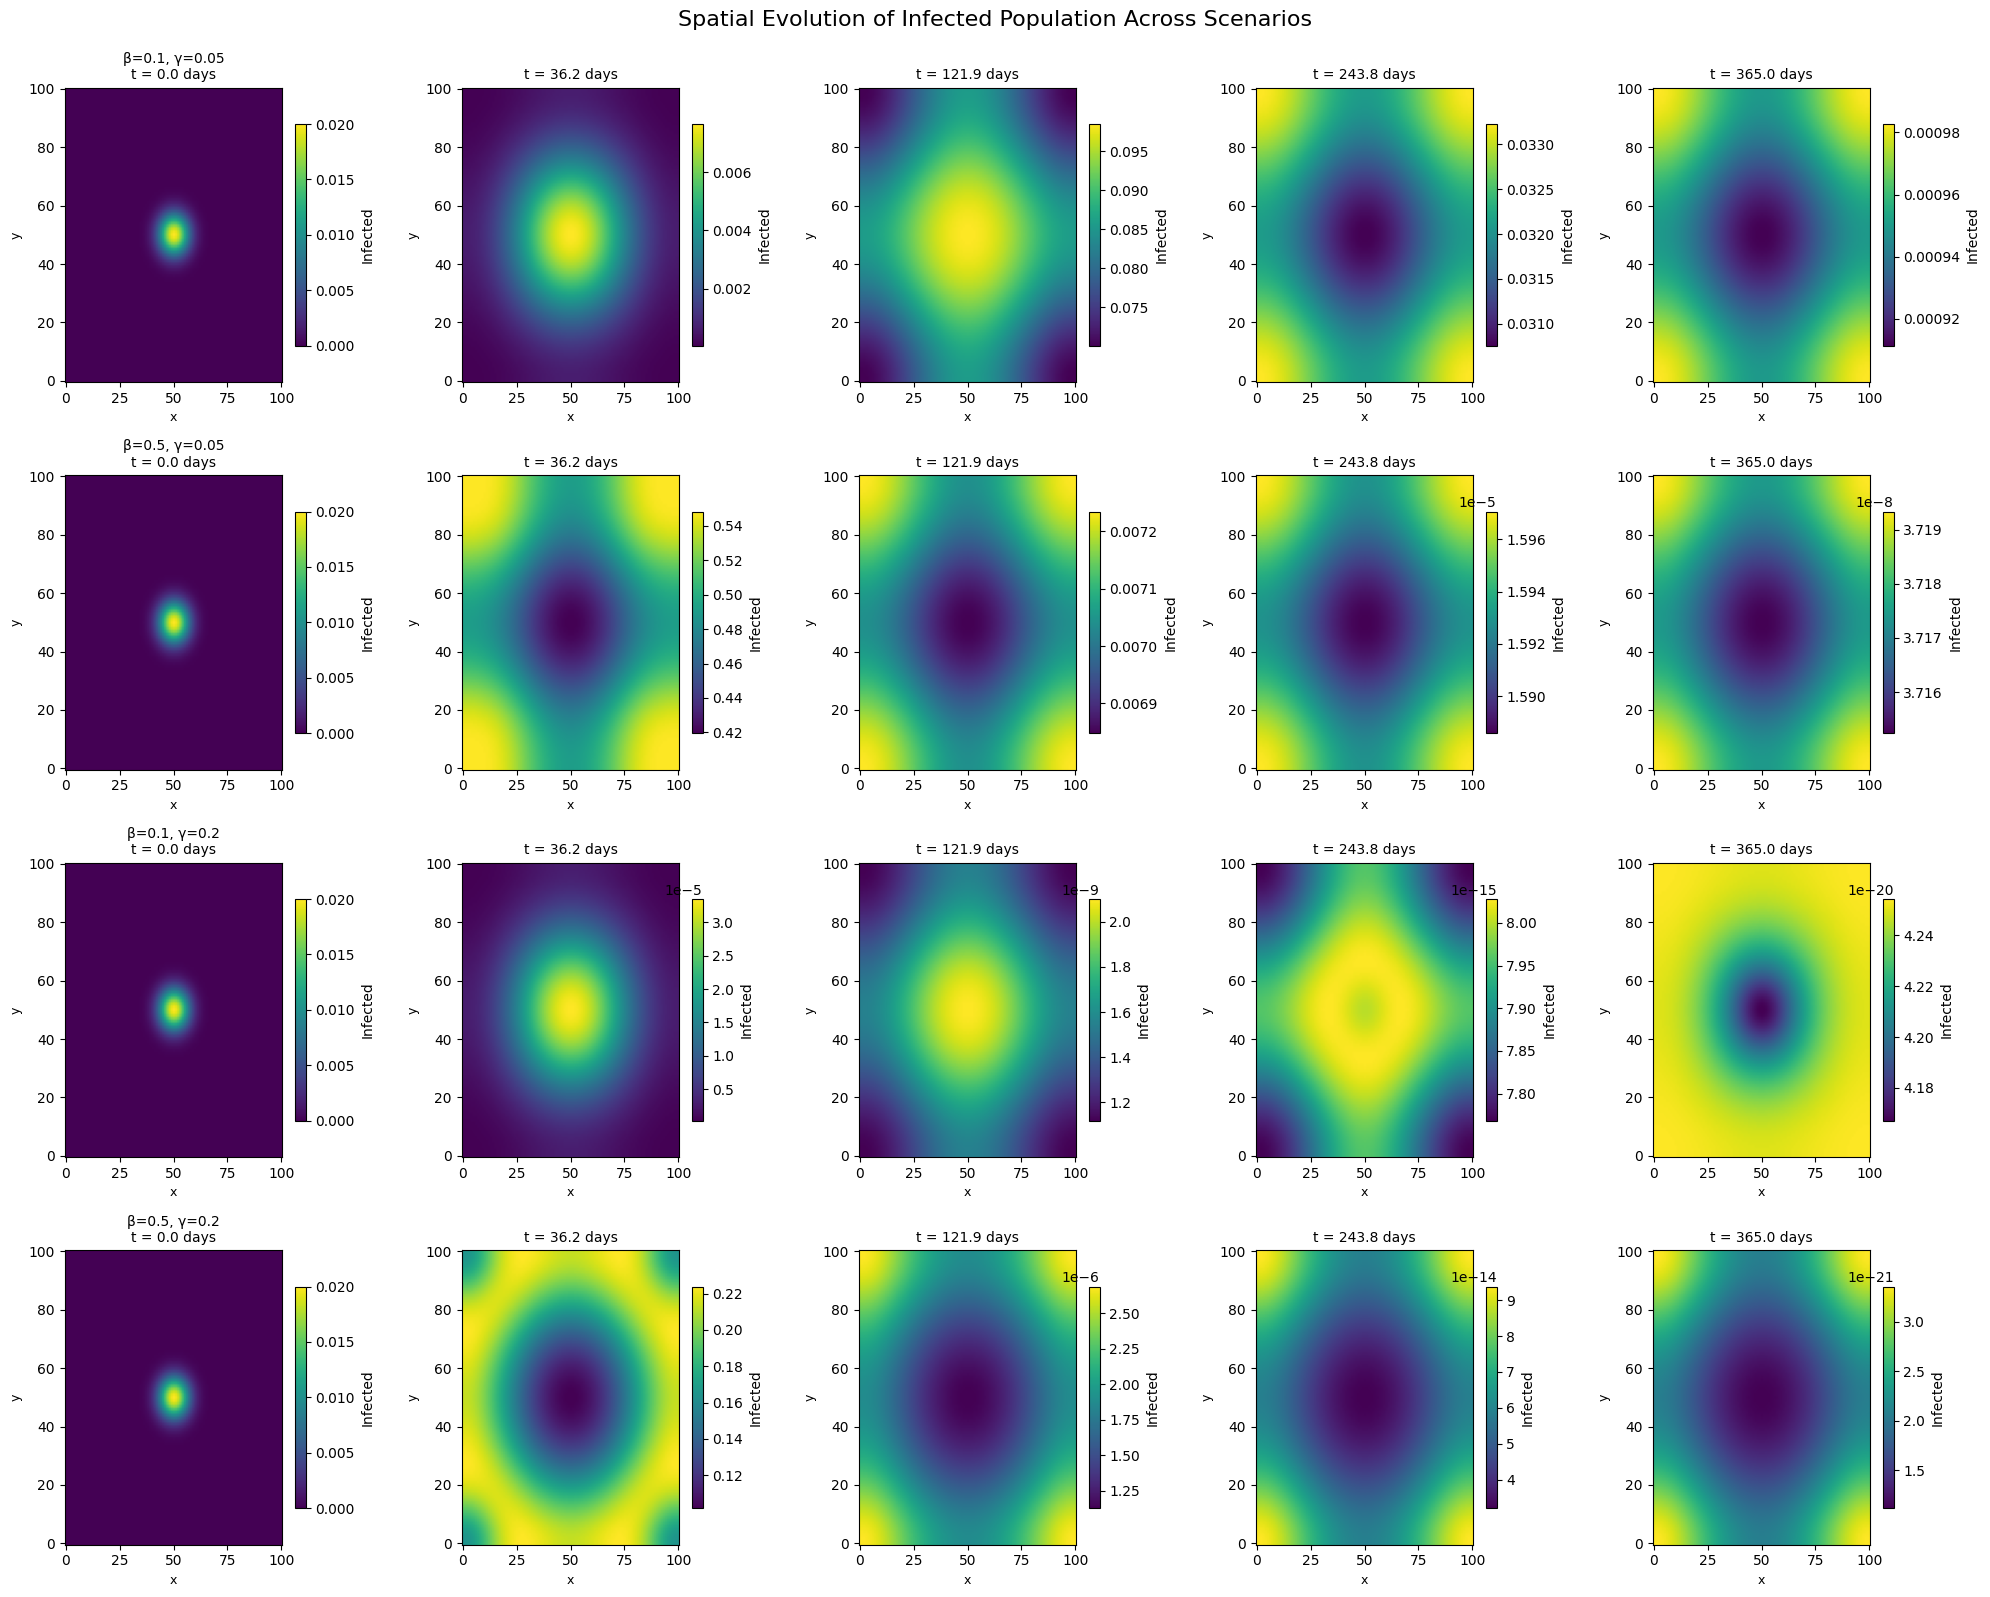
\includegraphics[keepaspectratio]{images/heatmap.png}}

}

\caption{Spatial snapshots at selected time points for all scenarios}

\end{figure}%




\end{document}
